
\subsection{Cross Sections as a function of the Transverse Momentum Imbalance parallel to the Muon Transverse Momentum }
%Results in \tkidpty 

Results for the differential cross section as a function of \tkidpty \ for interactions on the CH, C, H$_{2}$O, Fe, and Pb targets, respectively, are given in Fig.~\ref{figure:xsec_dpty}. 
%The data are represented by the black dots with error bars.  The expectation from the simulation (MnvGENIE) is given by the histograms and is broken down by the interaction process. 
This variable reflects changes to the outgoing proton energy after the interaction.  The negative tail indicates that the proton often loses energy traversing the nucleus.  The plots show that the tail increases in cross section relative to the peak as the nuclear size increases.  The MINERvA tune considerably underpredicts the cross section in the tail for the Pb target.  The uncertainties broken down by source for both the absolute cross sections and the cross section ratios as a function of \tkidpty\ can be found in Fig.~\ref{fig:xsec_err_dpty}.


% tki_dpty xsecs
\begin{figure}[h]  
	\centering
  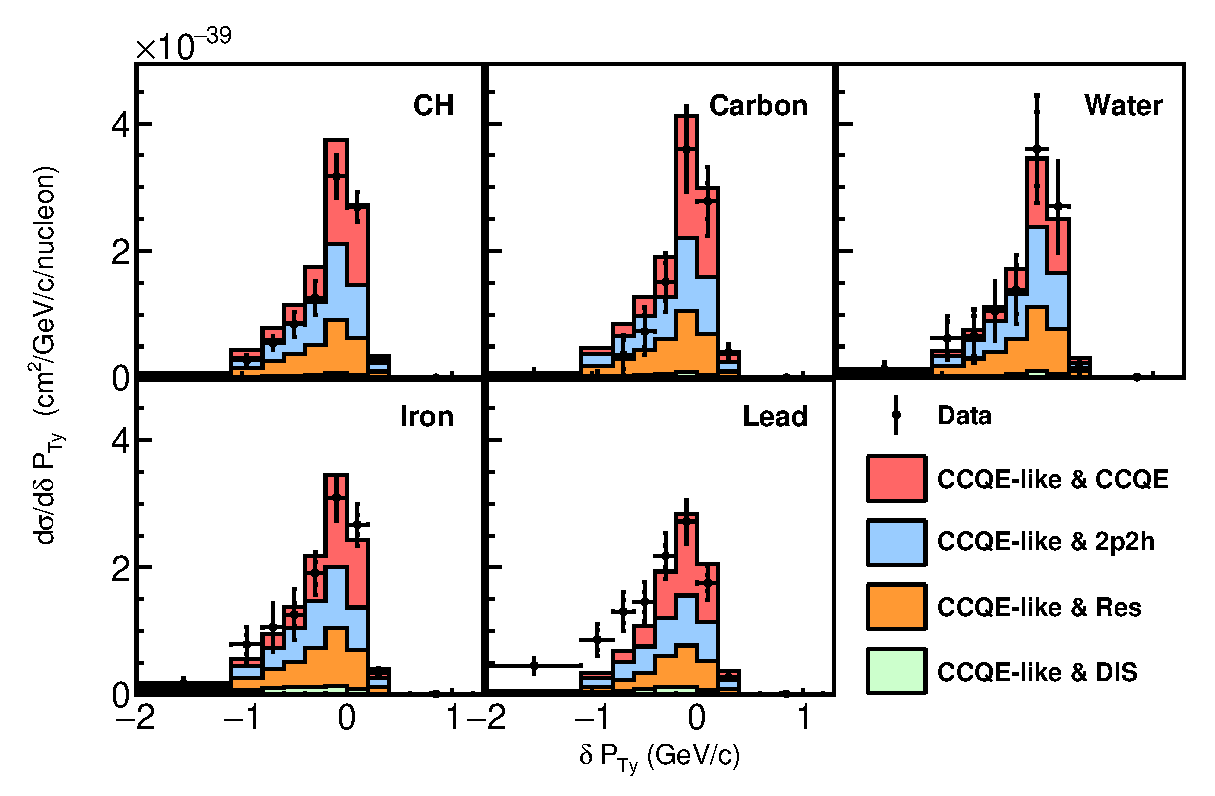
\includegraphics[width=\linewidth]{Figures/xsec_five_square/dpty.eps}
	\caption{The differential cross section as a function of \tkidpty \ for CH, C, H$_{2}$O, Fe, and Pb targets,along with the predictions for the different quasielastic-like signal processes.}
	\label{figure:xsec_dpty}
\end{figure}


The differential cross section as a function of \tkidpty \ for the different targets as compared to a range of models is given in Fig.~\ref{fig:models_dpty}. NEUT significantly overpredicts the cross section.  That overprediction is most pronounced for the larger targets, particularly in the tail where FSI is most important.  The hN versions of GENIE approach the prediction of NEUT in Pb.  The MINERvA tune and NuWro SF underpredict the cross section in the tail of \tkidpty \ for the Pb target. The \chisq\ between the cross sections and the models can be found in Table~\ref{tab:dpty}.

% comparisons to generators dpty
\begin{figure}
    \centering
        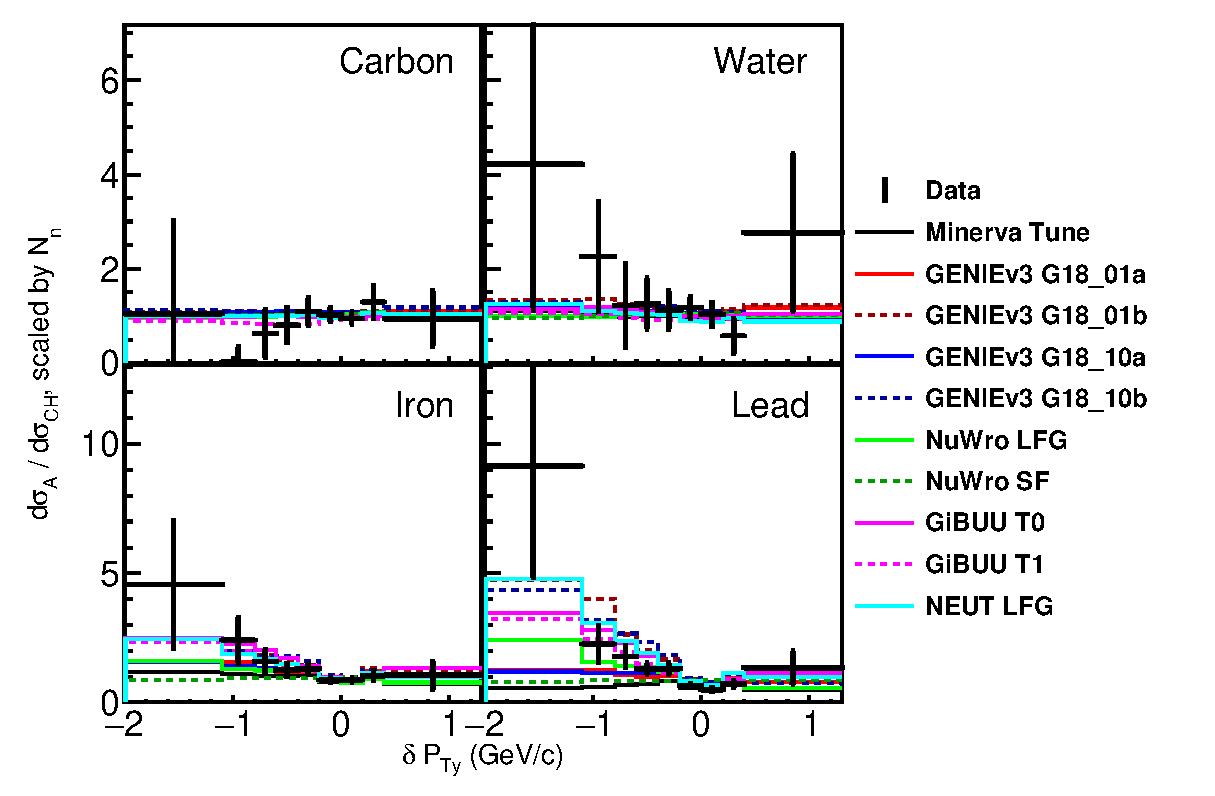
\includegraphics[width=\linewidth]{Figures/gencompare/dpty_4square.eps}
%    
     \caption{Cross section measurements and predictions as a function of \tkidpty\ for different targets and for a selection of different generator and model choices.}
    \label{fig:models_dpty}
\end{figure}


Figure~\ref{fig:ratiomodels_dpty} shows the differential cross-section ratio as a function of  \tkidpty \ for each nuclear target (C, H$_{2}$O, Fe, Pb) to that for scintillator. The models in general describe the data fairly well except in the tails of the larger targets where the model spread becomes pronounced.
The \chisq\ between the cross section ratios and the models can be found in Table~\ref{tab:dpty}.

\begin{figure}
    \centering
        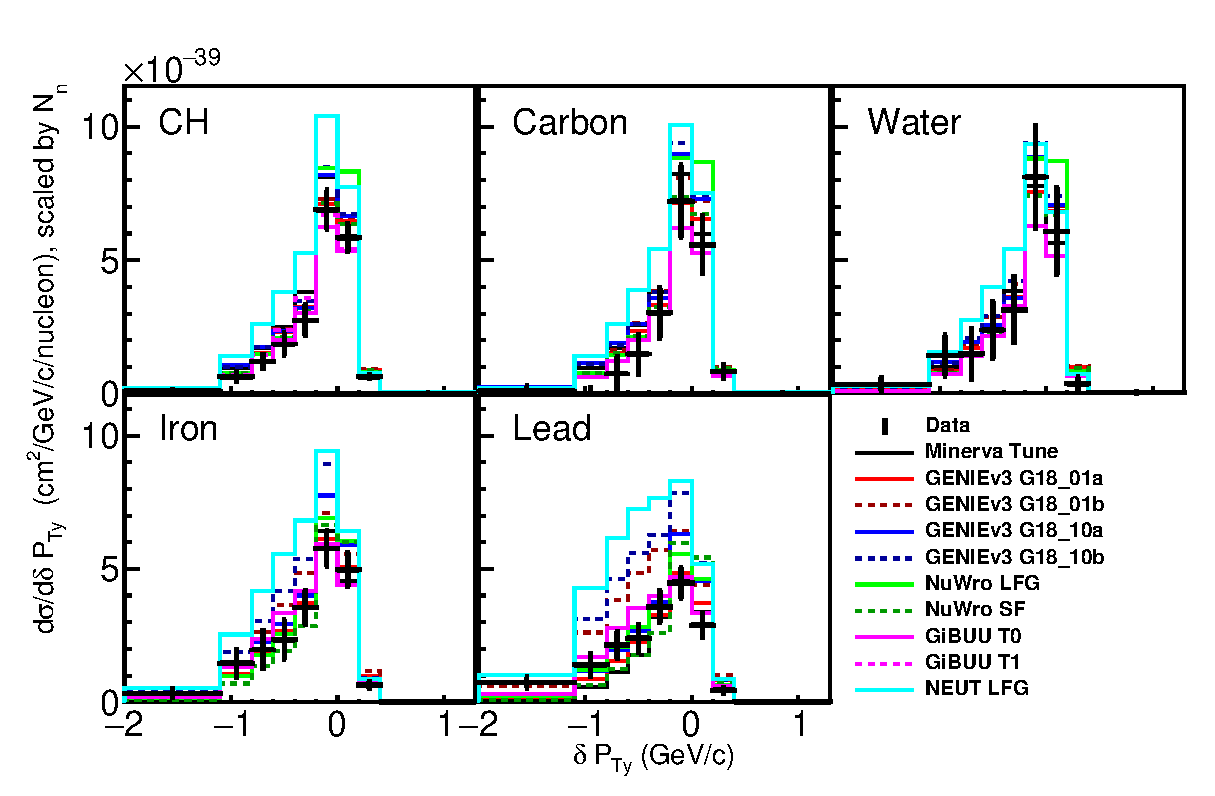
\includegraphics[width=\linewidth]{Figures/gencompare/dpty_5square.eps}
    \caption{\tkidpty\ cross-section ratio comparison for multiple targets.  Note that changes to the FSI model (GENIE ``a'' to ``b'')
     in GENIE change the cross section ratio at low values of \tkidpty\  more than changes to the 2p2h model (GiBUU T0 to GiBUU T1) or changes to the initial state (GENIE 1 to GENIE 10) or (NuWro LFG to NuWro SF).}
        \label{fig:ratiomodels_dpty}
\end{figure}
